\subsubsection{Connect \itwoc adapter to DCB master GBTx}
\label{sec:dcb-master-i2c}
A FFC breakout board is needed to connect \itwoc adapter to the DCB GBTx master.
Follow \autoref{fig:dcb_mc_i2c} to connect an external \itwoc adapter.

\begin{figure}[!ht]
\centering
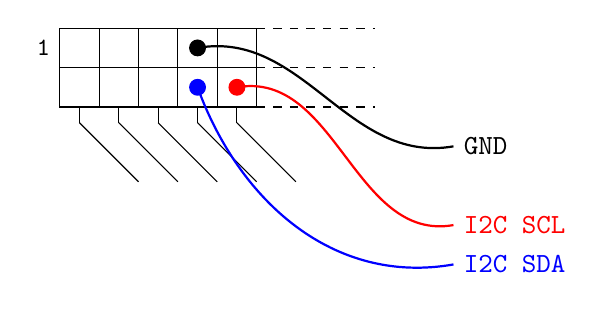
\begin{tikzpicture}
    % Pins
    \draw (0,0) rectangle (0.5,0.5);
    \draw (0.5,0) rectangle (1,0.5);
    \draw (1,0) rectangle (1.5,0.5);
    \draw (1.5,0) rectangle (2,0.5);
    \draw (2,0) rectangle (2.5,0.5);

    \draw (0,-0.5) rectangle (0.5,0);
    \draw (0.5,-0.5) rectangle (1,0);
    \draw (1,-0.5) rectangle (1.5,0);
    \draw (1.5,-0.5) rectangle (2,0);
    \draw (2,-0.5) rectangle (2.5,0);

    % Extension lines
    \draw [dashed] (2.5,0.5) -- (4,0.5);
    \draw [dashed] (2.5,0) -- (4,0);
    \draw [dashed] (2.5,-0.5) -- (4,-0.5);

    % Additional copper traces
    \draw (0.25,-0.5) -- (0.25,-0.7);
    \draw (0.75,-0.5) -- (0.75,-0.7);
    \draw (1.25,-0.5) -- (1.25,-0.7);
    \draw (1.75,-0.5) -- (1.75,-0.7);
    \draw (2.25,-0.5) -- (2.25,-0.7);

    \draw (0.25,-0.7) -- (1,-1.45);
    \draw (0.75,-0.7) -- (1.5,-1.45);
    \draw (1.25,-0.7) -- (2,-1.45);
    \draw (1.75,-0.7) -- (2.5,-1.45);
    \draw (2.25,-0.7) -- (3,-1.45);

    % Helper labels (imaginary)
    \coordinate (B) at (0,0.25);
    \node at (B) [left] {\small\texttt{1}};

    % GND
    \draw [black,fill] (1.75,0.25) circle [radius=0.1];
    \draw [thick] (1.75,0.25)
        to [out=10,in=190] (5,-1) node [right] {\texttt{GND}};

    % I2C SCL
    \draw [red,fill] (2.25,-0.25) circle [radius=0.1];
    \draw [red,thick] (2.25,-0.25)
        to [out=10,in=190] (5,-2) node [right] {\texttt{I2C SCL}};

    % I2C SDA
    \draw [blue,fill] (1.75,-0.25) circle [radius=0.1];
    \draw [blue,thick] (1.75,-0.25)
        to [out=-70,in=190] (5,-2.5) node [right] {\texttt{I2C SDA}};
\end{tikzpicture}
\caption{
    \itwoc adapter needs to be connected on DCB master FFC breakout board.
    Pay attention to the implied orientation of the breakout board, as it is
    helpful to locate pin 1.
}
\label{fig:dcb_mc_i2c}
\end{figure}
